\documentclass{gapd}

\Type{自助出版}
\Title{平行可變的間隙限制最長共同子序列 \\ Parallel Variable Gapped Longest Common Sequence}

\Author{Shiang-Yun Yang}{National Taiwan University}

\Author{Morris Yang}{National Taiwan University}

\Author{Stephanie Dola}{National Taiwan University}

\Abstract{可變的間隙限制最長同子序列應用於基因、分子生物學中。在之前所有的研究,已經提出在 $O(nm \alpha(n))$ 時間內的算法,其中使用了高效的遞增後綴最大值詢問,可以在 $O(\alpha(n))$ 解決每一詢問。原先的序列算法無法以直觀的方式平行,我們修改了原本算法的資料結構,並且提出平行版本的遞增任意區間最大值詢問,平行的運行時間為 $O(nm / p + n \log n)$。在單一處理器上,理論的時間複雜度可以達到 $O(nm)$ 勝過於先前的研究。

\begin{quote}\itshape
  「專注於足下,才能走得更遠」 -- 真正的名言是「千里之行,始於足下」,然而某一次意外地把足下放在前面,就在人生上留下了更多的污點。
\end{quote}

}

\Issue{1}{1}{2017}
%\Pages{35}{37}

\begin{document}
\maketitle

\section{介紹} %Introduction
\label{sec:Introduction}

最長同子序列 (\emph{longest common subsequence}) (LCS)廣泛地使用在各個應用上。在多核心平台下,大多數的研究專注於如何高效率地在波前平行,而 Jiaoyun Yang ~\cite{jiaoyun} 提出的論文中改變一般的 LCS 遞迴定義以得到更好快取使用率。這裡,我們使用相關的理論來改善在 Iliopoulos ~\cite{iliopoulos} 提及的約束條件下的 LCS,如 \emph{fixed gap LCS } (FGLCS)要求任兩個挑選的距離在相對應的另一個字串中相等,同時距離最大為 $k+1$,可在時間複雜度在 $O(nm)$ 內解決,其中 $n$, $m$ 分別為兩個輸入的字串長度。

在眾多的約束條件類型中,我們將在這篇論文針對 \emph{variable gap LCS} (VGLCS) 進行探討。在 VGLCS 中,對各個不同的位置提供約束限制,如目前給定兩個字串 $A = \tt{RCLPCRR}$, $B = \tt{RPPLCPLRC}$,各自的約束限制為 $G_A = [2, 3, 0, 0, 3, 2, 2]$ 和 $G_B = [2, 0, 0, 0, 3, 0, 0, 2, 3]$,其中 $G_A(i)$ 表示當挑選第 $i$ 個位置時,與前一個挑選的位置最多差 $G_A(i)+1$,挑選的方式如圖 ~\ref{fig:VGLCSex}。這個問題已在 Yung-Hsing Peng ~\cite{yunghsing} 的論文針對 VGLCS 提出 $O(nm \alpha(n))$ 的解法。

這一篇論文,我們將在第 \ref{??} 節部分將 Yung-Hsing Peng ~\cite{yunghsing} 提出的算法進行平行化。次著,在第 \ref{??} 節,我們將藉由快取忘卻 (cache-oblivious) 技術,在實作上提供更好的效能。接著,在第 \ref{??} 節,在理論分析上提供易平行且時間複雜度 $O(nm)$ 的設計。最後,我們總結實驗結果與理論實務上的差異。

\begin{figure*}[!thb]
  \centering
  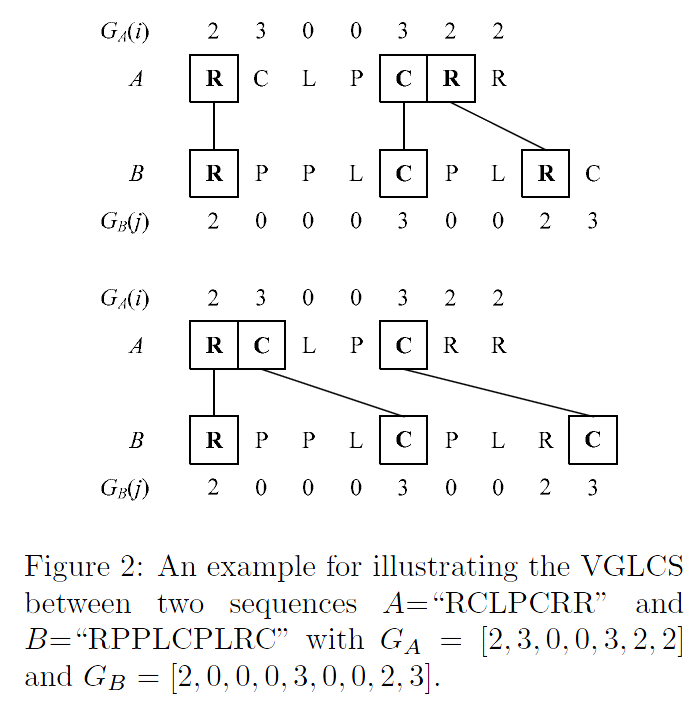
\includegraphics[height=5cm]{figure/fig-VGLCS-ex.png} % width=\linewidth,
  \caption{簡單的 VGLCS 於兩個序列 $A = \tt{RCLPCRR}$, $B = \tt{RPPLCPLRC}$,各自的約束限制為 $G_A = [2, 3, 0, 0, 3, 2, 2]$ 和 $G_B = [2, 0, 0, 0, 3, 0, 0, 2, 3]$,的其中幾個可挑選的方案}
  \label{fig:VGLCSex}
\end{figure*}

\section{平行化序列算法}
\label{sec:Ambiguity}

在 $O(nm)$ 的序列算法中 (參考圖 ~\ref{VGLCSalgo}),我們發現算法如大多數的變型 LCS 相同,依賴左上角區塊的狀以轉移當前狀態,大量的資料依賴性不易於細粒度平行。使用波前運行平行是一種常見的解決方案,由於這種平行對於運行時的快取不友善 (cache-unfriendly),所以在 Saeed Maleki~\cite{saeed} 論文中提到如何使用 Rank Convergence 的特殊性質,拓展出更高平行度來解決動態規劃的相關問題。

序列算法的空間複雜度為 $O(nm)$。若使用波前平行,需要同時維護橫向的所有狀態,需要多付出一倍的空間量。若加入 Rank Convergence 的想法拓展出,勢必要記錄轉移的狀態,需要耗費更多的記憶體空間,用以在最後階段合併所用。

這裡我們著手設計算法空間複雜度常數小,並且針對快取友善。從序列算法中,發現在橫向查找中使用 $O(\alpha(n))$ 操作的後綴最大值查找,這部分難以平行化。為了消除資料相依性,我們找到幾種區間詢問的替代方案。如 

\begin{itemize}
  \item Binary Indexed Tree -- $O(\log n)$
  \item Range Tree -- $O(\log n)$
  \item Sparse Table -- $O(n \log n) -- O(1)$
\end{itemize}

根據 VGLCS 動態規劃時的單調性質,可以使用 Van Emde Boas Tree 作為輔助資料結構在 $O(\log \log n)$ 時間內完成操作。其中 Sparse Table 是我們認為最好的替代方案,其整合後的平行算法如圖 ~\ref{??},在平行的時間複雜度為 $O(n^2 / p + n \log n)$,其中 $p$ 為處理器個數。

\begin{figure*}[!thb]
  \centering
  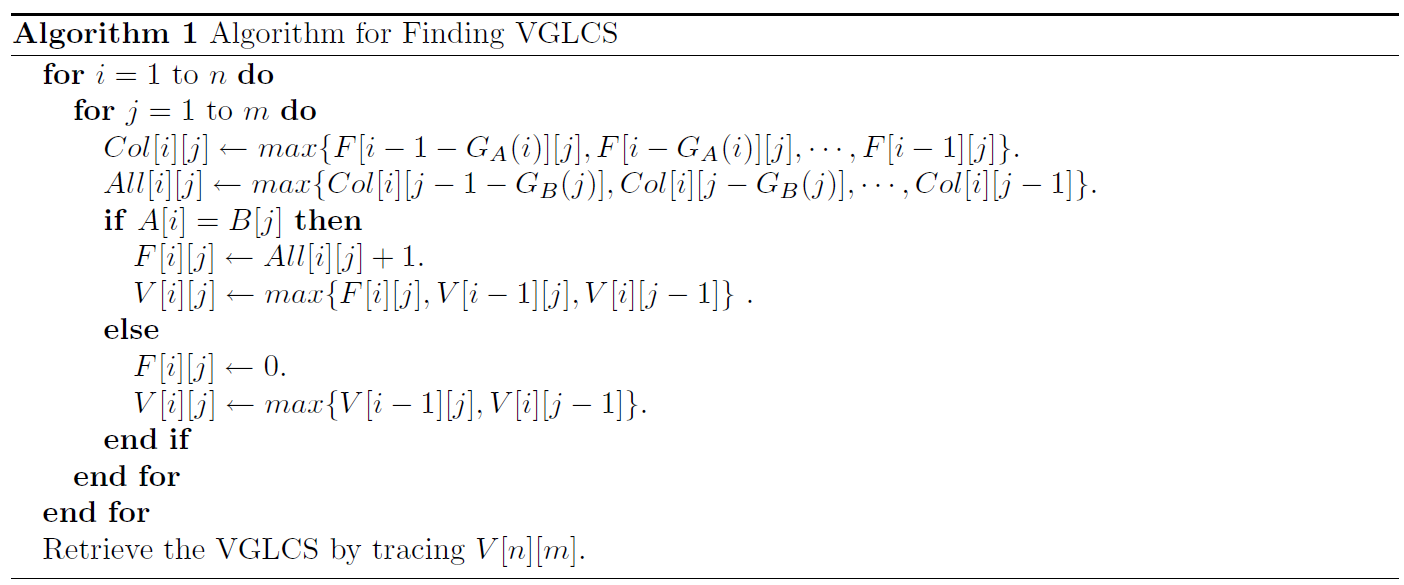
\includegraphics[height=5cm]{figure/fig-VGLCS-algo.png} % width=\linewidth,
  \caption{Yung-Hsing Peng ~\cite{yunghsing} 提出的原生算法}
  \label{fig:VGLCSalgo}
\end{figure*}

\section{結論}
\label{sec:Conclusion}

\section*{致謝}

特別感謝某某

\section*{References}

\begin{thebibliography}{4}

\bibitem{jiaoyun} Jiaoyun Yang, Yun Xu, Yi Shang, `An Efficient Parallel Algorithm for Longest Common Subsequence Problem on GPUs', Proceedings of the World Congress on Engineering, 2010, vol.~I 

\bibitem{iliopoulos} C. S. Iliopoulos and M. S. Rahman, `Algorithms for computing variants of the longest common subsequence problem', Theoretical Computer Science, 2008, vol.~395, pp. 255--267

\bibitem{yunghsing} Yung-Hsing Peng and Chang-Biau Yang, The Longest Common Subsequence Problem with Variable Gapped Constraints

\bibitem{saeed} Saeed Maleki, `Efficient Parallelization Using Rank Convergence in Dynamic Programming Algorithm', Microsoft, 2016

\end{thebibliography}

\Note{BlueNoteBackground}{%
  {\bf Cameron Browne} is a Vice-Chancellor's Senior Research Fellow
  at QUT, Brisbane, Australia, whose research interests include artificial intelligence and automated game design.\\
  {\bf Address:} School of EECS, Science and Engineering Faculty, QUT,
  Brisbane, 4001, Australia.\\
  {\bf Email:} c.browne@qut.edu.au
%
}

\end{document}
